\documentclass[tikz,border=2pt]{standalone}
\usepackage{amsmath}
\usetikzlibrary{shapes.geometric}
\definecolor{nuzero}{RGB}{166,213,226}
\definecolor{nuone}{RGB}{220,139,142}
\definecolor{metal}{RGB}{180,159,205}
\definecolor{bulk}{RGB}{74,58,126}
\definecolor{capcolor}{RGB}{189,89,43}
\definecolor{defect}{RGB}{55,55,60}
\definecolor{ink}{RGB}{38,38,42}
\definecolor{datablue}{RGB}{0,87,184}
\definecolor{datablack}{RGB}{0,0,0}
\definecolor{datared}{RGB}{198,40,40}
\begin{document}
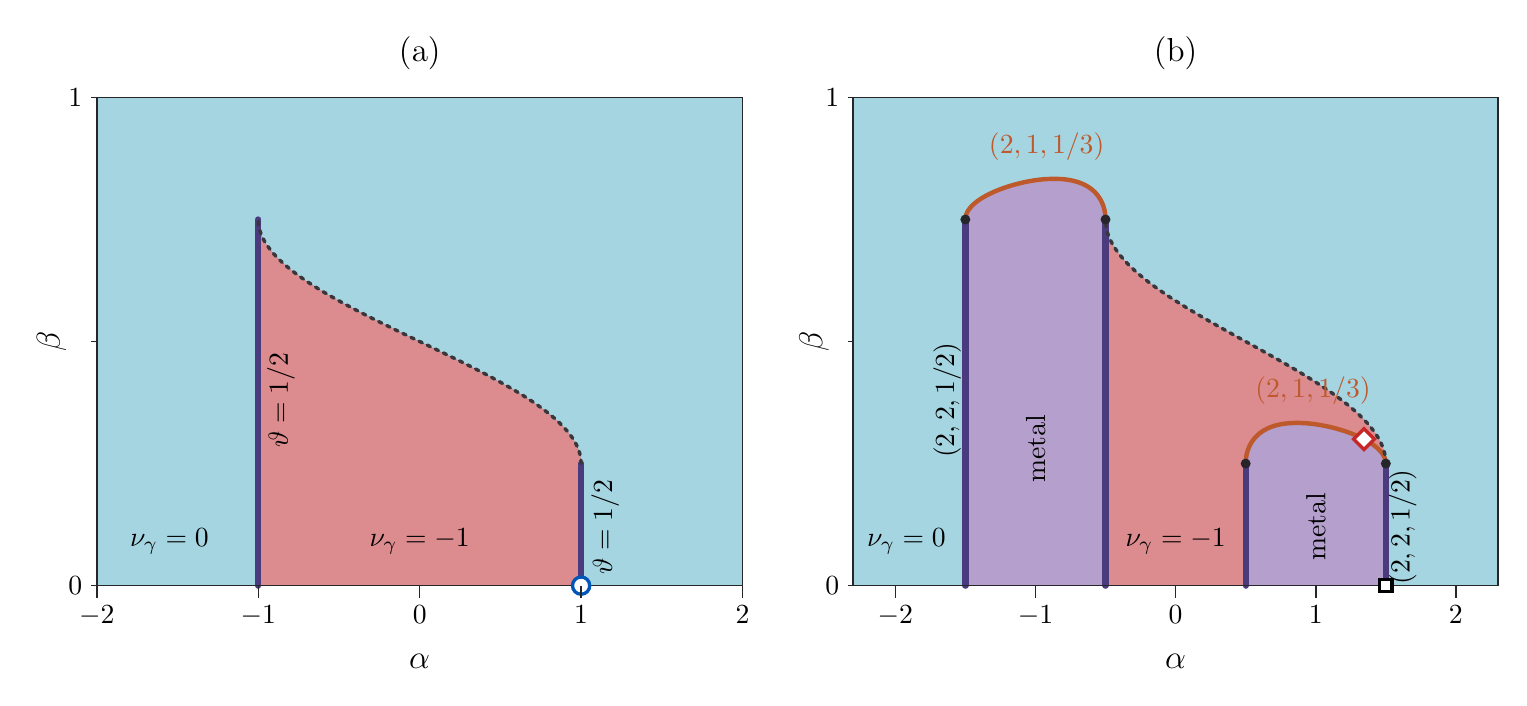
\begin{tikzpicture}[
 every node/.style={font=\normalsize},
 critical/.style={bulk,line width=2.3pt,line cap=round,line join=round},
 capline/.style={capcolor,line width=1.6pt,line cap=round,line join=round},
 defectline/.style={defect,dotted,line width=1.25pt,line cap=round},
 axis/.style={ink,line width=.55pt}]
\begin{scope}[x=2.05cm,y=6.2cm]
 \fill[nuzero] (-2,0) rectangle (2,1);
 \path[fill=nuone] (-1,0)--(1,0)--(1,.25)
  --plot[domain=.25:.75,samples=220,variable=\t] ({sin(360*\t)},{\t})
  --(-1,.75)--cycle;
 \draw[critical] (1,0)--(1,.25);
 \draw[critical] (-1,0)--(-1,.75);
 \draw[defectline] plot[domain=.25:.75,samples=220,variable=\t]
  ({sin(360*\t)},{\t});
 \node at (-1.55,.09) {$\nu_\gamma=0$};
 \node at (0,.09) {$\nu_\gamma=-1$};
 \node[rotate=90] at (-.86,.38) {$\vartheta=1/2$};
 \node[rotate=90] at (1.15,.12) {$\vartheta=1/2$};
 \draw[axis] (-2,0) rectangle (2,1);
 \node[circle,inner sep=2.2pt,line width=1.2pt,
       draw=datablue,fill=white] at (1,0) {};
 \foreach \x in {-2,-1,0,1,2}{
  \draw[axis] (\x,0)--++(0,-.025);
  \node[below] at (\x,-.02) {$\x$};}
 \foreach \y/\lab in {0/0,.5/{},1/1}{
  \draw[axis] (-2,\y)--++(-.035,0);
  \node[left] at (-2.03,\y) {$\lab$};}
 \node[font=\large,below] at (0,-.12) {$\alpha$};
 \node[font=\large,rotate=90] at (-2.28,.5) {$\beta$};
 \node[font=\large] at (0,1.09) {(a)};
\end{scope}

\begin{scope}[shift={(9.6cm,0)},x=1.78cm,y=6.2cm]
 \def\M{.5}
 \def\A{2.3}
 \pgfmathsetmacro{\Btip}{.25+asin(\M)/360}
 \fill[nuzero] (-\A,0) rectangle (\A,1);
 \path[fill=nuone] ({-1+\M},0)--({1-\M},0)--({1-\M},.25)
  --plot[domain=.25:.75,samples=220,variable=\t]
    ({sin(360*\t)+\M},{\t})--({-1+\M},.75)--cycle;
 \path[fill=metal] ({1-\M},0)--({1+\M},0)--({1+\M},.25)
  --plot[domain=.25:\Btip,samples=140,variable=\t]
    ({sin(360*\t)+sqrt(max(0,\M*\M-pow(cos(360*\t),2)))},{\t})
  --plot[domain=\Btip:.25,samples=140,variable=\t]
    ({sin(360*\t)-sqrt(max(0,\M*\M-pow(cos(360*\t),2)))},{\t})--cycle;
 \path[fill=metal] ({-1-\M},0)--({-1+\M},0)--({-1+\M},.75)
  --plot[domain=.75:{.5+\Btip},samples=140,variable=\t]
    ({sin(360*\t)+sqrt(max(0,\M*\M-pow(cos(360*\t),2)))},{\t})
  --plot[domain={.5+\Btip}:.75,samples=140,variable=\t]
    ({sin(360*\t)-sqrt(max(0,\M*\M-pow(cos(360*\t),2)))},{\t})--cycle;
 \foreach \x/\b in {{1-\M}/.25,{1+\M}/.25,{-1-\M}/.75,{-1+\M}/.75}
  {\draw[critical] (\x,0)--(\x,\b);}
 \draw[capline]
  plot[domain=.25:\Btip,samples=140,variable=\t]
   ({sin(360*\t)-sqrt(max(0,\M*\M-pow(cos(360*\t),2)))},{\t})
  --plot[domain=\Btip:.25,samples=140,variable=\t]
   ({sin(360*\t)+sqrt(max(0,\M*\M-pow(cos(360*\t),2)))},{\t});
 \draw[capline]
  plot[domain=.75:{.5+\Btip},samples=140,variable=\t]
   ({sin(360*\t)+sqrt(max(0,\M*\M-pow(cos(360*\t),2)))},{\t})
  --plot[domain={.5+\Btip}:.75,samples=140,variable=\t]
   ({sin(360*\t)-sqrt(max(0,\M*\M-pow(cos(360*\t),2)))},{\t});
 \draw[defectline] plot[domain=.25:.75,samples=220,variable=\t]
  ({sin(360*\t)+\M},{\t});
 \foreach \x/\y in {.5/.25,1.5/.25,-1.5/.75,-.5/.75}
  {\fill[ink] (\x,\y) circle[radius=1.8pt];}
 \node at (-1.92,.09) {$\nu_\gamma=0$};
 \node at (0,.09) {$\nu_\gamma=-1$};
 \node[rotate=90] at (-1,.28) {metal};
 \node[rotate=90] at (1,.12) {metal};
 \node[rotate=90] at (-1.63,.38) {$(2,2,1/2)$};
 \node[rotate=90] at (1.62,.12) {$(2,2,1/2)$};
 \node[capcolor] at (-.92,.9) {$(2,1,1/3)$};
 \node[capcolor] at (.98,.4) {$(2,1,1/3)$};
 \draw[axis] (-\A,0) rectangle (\A,1);
 \pgfmathsetmacro{\Adata}{sin(360*.30)+sqrt(\M*\M-pow(cos(360*.30),2))}
 \node[rectangle,inner sep=2.2pt,line width=1.2pt,
       draw=datablack,fill=white] at (1.5,0) {};
 \node[diamond,aspect=1,inner sep=2.0pt,line width=1.2pt,
       draw=datared,fill=white] at (\Adata,.30) {};
 \foreach \x in {-2,-1,0,1,2}{
  \draw[axis] (\x,0)--++(0,-.025);
  \node[below] at (\x,-.02) {$\x$};}
 \foreach \y/\lab in {0/0,.5/{},1/1}{
  \draw[axis] (-\A,\y)--++(-.035,0);
  \node[left] at (-\A-.03,\y) {$\lab$};}
 \node[font=\large,below] at (0,-.12) {$\alpha$};
 \node[font=\large,rotate=90] at (-\A-.28,.5) {$\beta$};
 \node[font=\large] at (0,1.09) {(b)};
\end{scope}
\end{tikzpicture}
\end{document}
